
\section{Problem Statement}
Industry 4.0 has brought together traditional operational technology and IT systems, resulting in new attack vectors \cite{dietzUnleashingDigitalTwin2020}. The literature review has also revealed two major challenges in Industry 4.0: speed and security. For example, in the power automation system, the minimum acceptable time between fault detection and control sent to the power station must be as low as 4ms \cite{rajkumar_cyber_2020} in order to ensure a timely response. Besides, Digital Twin is a trending topic that started being used in Industry 4.0 for various applications including monitoring, testing, and simulation of operations. However, our literature review reveals that most researchers either recommend a traditional encryption algorithm to secure the communication channel between IoT devices. On the other hand, from a security perspective, computational and power limitations make it difficult for (I)IoT sensors to use traditional encryption algorithms. Due to these two reasons, it is essential to explore and implement lightweight encryption schemes that meet the security requirements while maintaining the necessary speed and efficiency of these systems.

\section{Proposed Solution}
The (Industrial) Internet of Things ((I)IoT) devices are low-power and resource-constrained, which makes them incapable of running traditional cryptographic schemes such as AES. Regardless, these devices are widely used across a range of Industry 4.0 sectors, such as manufacturing, transportation, health, and power grids, for various applications. In addition, IoT sensors are an integral part of Digital Twin technology, in which they are used to collect and send data over wired or wireless channels.

In this paper, we propose efficient and lightweight cryptographic encryption and authentication schemes to enhance the security of the communication channel between the Digital Twin and its physical components over the MQTT protocol using a technique called payload encryption.

\textbf{\textit{Why Lightweight encryption}}:
Lightweight cryptography algorithms are designed to be efficient and fast, making them suitable for use in resource-constrained environments such as (I)IoT devices and embedded systems.
These algorithms can be used to secure data at transit and rest in (I)IoT devices, ensuring the confidentiality, integrity, and authenticity of data. Furthermore, they are essential in applications where \textbf{real-time} data processing and \textbf{low latency} are critical requirements.

The following diagrams \ref{fig:ps-archi} show the general system overview of our proposed solution. 

\begin{figure}[H]
    \centering
    \includesvg[width=\textwidth, height=40cm]{images/svg/ps-scheme-final.svg}
    % 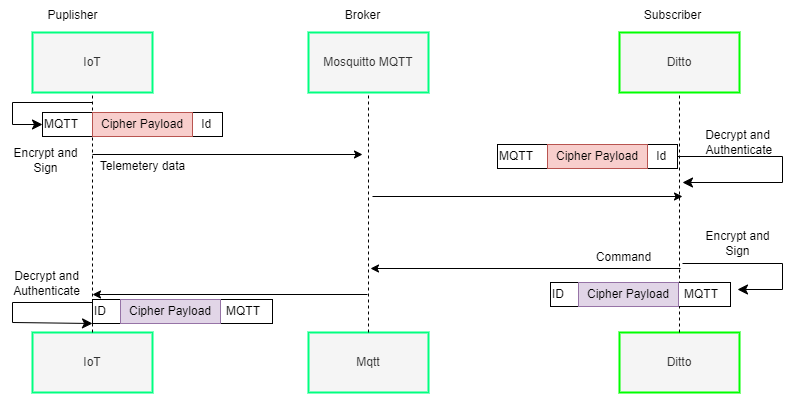
\includegraphics[width=\textwidth]{images/fp/payloadenc.drawio.png}
    \caption{System Overview of Proposed Solution}
    \label{fig:ps-archi}
\end{figure}







\section{Implementation Methodology}
To address research questions three (RQ3) and four (RQ4), we will select and implement an authentication/encryption scheme on
an open-source Digital Twin platform called Ditto and on one of a micro-controller device called ESP32. The authentication/encryption scheme is based on a lightweight cryptographic algorithm standardized by NIST. 

Ditto is an open-source framework developed and maintained by Eclipse Foundation to facilitate the interaction between Digital Twin and IoT devices\cite{noauthor_eclipse_nodate}. On the other hand, ESP32 is a micro-controller chip manufactured by the Espressif system. 

To answer the last research question(RQ4), we will evaluate the performance of proposed scheme implementation in terms of power consumption, execution time, and storage complexity. 

